You are building a sensor that can detect the light in a room. Shown below is a simplified version of the main circuit for the sensor. Instead of using a normal voltage source, we are using a voltage source that changes its value based on the luminosity of the light source. Specifically, we know that the voltage $V_p$ changes as a function of the luminosity, $V_p = f(L_p)$. However, the label on the voltage source is scratched, so we'd like to recover $f$. \\ \\
We attach an ammeter (a device that measures current) as shown in the circuit below, and we would like to recover $f$ based on how the ammeter reading changes as we change the brightness of a light source directly pointed at the voltage source (thereby changing $V_p$).

\begin{figure}[H]
    \centering
    \begin{circuitikz}[american]
        \draw (0,0) to[pvsource, l=$V_p$](0,3) -- (1,3) to[ammeter](2, 3)--(3, 3) to[R=$R_1$] (3,0) -- (0,0);
        \draw (-0.5, 1) node{$-$};
        \draw (-0.5, 2) node{$+$};
        \draw (3,3) -- (5,3) to[R=$R_2$](5,0) -- (2,0);
        \draw (0,0) -- (0, -0.5) node[ground]{};
    \end{circuitikz}
\end{figure}

\begin{enumerate}
    \item To get started, label the positive and negative terminals of the resistors and the ammeter based on the passive sign convention and how we've labeled the voltage source. To ensure consistency,  assume current comes out of the positive terminal of the voltage source and flows into the positive terminal of all other circuit elements.

    \note{
        Encourage the students to follow the direction of the current and the label and positve and negative terminals as instructed in the question.
    }

    \sol{
        {
            \color{blue}
            \begin{figure}[H]
                \centering
                \begin{circuitikz}[american]
                    \draw (0,0) to[pvsource, l=$V_p$](0,3) -- (1,3) to[ammeter](2, 3)--(3, 3) to[R=$R_1$] (3,0) -- (0,0);
                    \draw (-0.5, 1) node{$-$};
                    \draw (-0.5, 2) node{$+$};
                    \draw (3,3) -- (5,3) to[R=$R_2$](5,0) -- (2,0);
                    \draw (0,0) -- (0, -0.5) node[ground]{};
                    \draw (3.5, 1) node{$-$};
                    \draw (3.5, 2) node{$+$};
                    \draw (5.5, 1) node {$-$};
                    \draw (5.5, 2) node{$+$};
                    \draw (1, 3.5) node {$+$};
                    \draw (2, 3.5) node {$-$};
                    \draw (0,0) -- (0, -0.5) node[ground]{};
                \end{circuitikz}
            \end{figure}
        }
    }

    \item Let the current reading measured by the ammeter be $i$. Express $i$ as a function of $V_p$, $R_1$, and $R_2$.

    \note{
        Encourage students to think about equivalence within the circuit, namely parallel. It is also a good idea to use a simple KCL and KVL on this question to see how parallel circuit divides the current (compared to series circuit that acts as a voltage divider).
    }

    \sol{
        We can see that $R_1$ and $R_2$ are in parallel, hence sharing the same voltage as $V_p$ and act as a current divider. Using Ohm's Law, we have:
        $$i = i_1 + i_2 = \frac{V_p}{R_1} + \frac{V_p}{R_2}.$$
    }
    \item Suppose $R_1 = 2\Omega$ and $R_2 = 3\Omega$, and we have the following scattering plot of $L_p$ versus $i$ based on the readings from the ammeter:
    \begin{figure}[H]
        \centering
        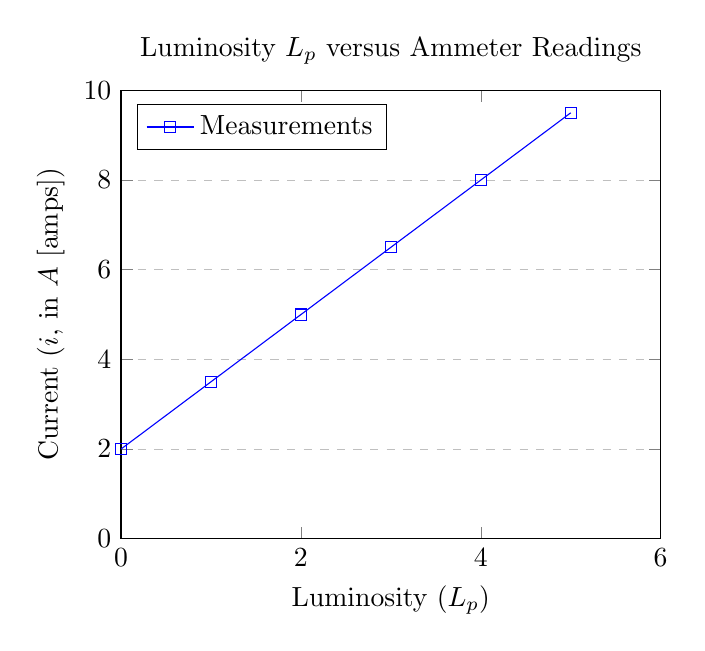
\begin{tikzpicture}
            \begin{axis}[
                title={Luminosity $L_p$ versus Ammeter Readings},
                xlabel={Luminosity ($L_p$)},
                ylabel={Current ($i$, in $A$ [amps])},
                xmin=0, xmax=6,
                ymin=0, ymax=10,
                xtick={0,2,4,6},
                ytick={0,2,4,6,8,10},
                legend pos=north west,
                ymajorgrids=true,
                grid style=dashed,
            ]
    
            \addplot[
                color=blue,
                mark=square,
                ]
                coordinates {
                (0,2)(1,3.5)(2,5)(3,6.5)(4,8)(5,9.5)
                };
                \legend{Measurements}
    
            \end{axis}
        \end{tikzpicture}
    \end{figure}
    \begin{enumerate}
        \item In the grid below, plot out the $i$ versus $V_p$ graph. Make sure to label at least 2 points on the graph.

        \note{
            Be sure to enforce the idea that in this class, for a fixed constant resistor, $I$ versus $V$ will always constant as well (the plot should always look like a slanted line with positive slope that passes through the origin). This is the essence of Ohm's Law and it won't be affected by any external settings (no matter how complicated they are).
        }

        \begin{figure}[H]
            \centering
            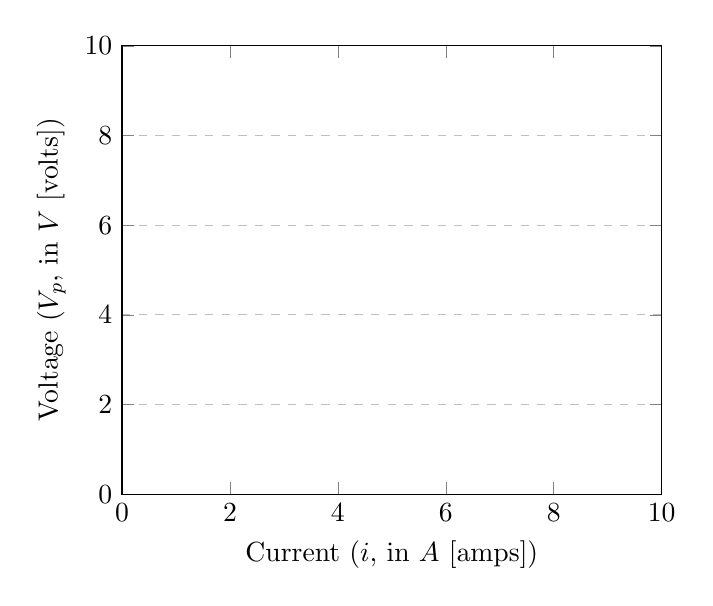
\begin{tikzpicture}
                \begin{axis}[
                    xlabel={Current ($i$, in $A$ [amps])},
                    ylabel={Voltage ($V_p$, in $V$ [volts])},
                    xmin=0, xmax=10,
                    ymin=0, ymax=10,
                    xtick={0,2,4,6,8,10},
                    ytick={0,2,4,6,8,10},
                    legend pos=north west,
                    ymajorgrids=true,
                    grid style=dashed,
                ]
                \end{axis}
            \end{tikzpicture}
        \end{figure}

        \sol{
        $V_p = i \cdot \frac{R_1R_2}{R_1 + R_2} = 1.2i$.

        \begin{figure}[H]
            \centering
            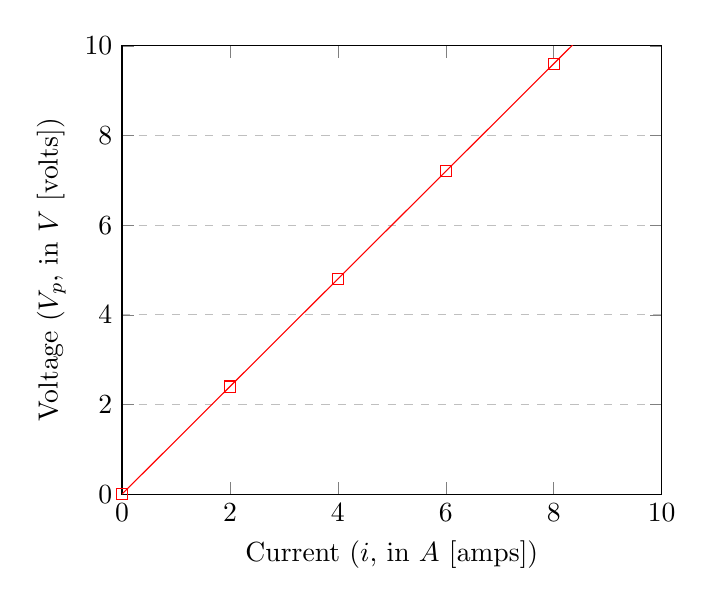
\begin{tikzpicture}
                \begin{axis}[
                    xlabel={Current ($i$, in $A$ [amps])},
                    ylabel={Voltage ($V_p$, in $V$ [volts])},
                    xmin=0, xmax=10,
                    ymin=0, ymax=10,
                    xtick={0,2,4,6,8,10},
                    ytick={0,2,4,6,8,10},
                    legend pos=north west,
                    ymajorgrids=true,
                    grid style=dashed,
                ]

                \addplot[
                color=red,
                mark=square,
                ]
                coordinates {
                (0,0)(2,2.4)(4,4.8)(6,7.2)(8,9.6)(10,12)
                };
                \end{axis}
            \end{tikzpicture}
        \end{figure}
        }
        \item Recover the expression for $V_p = f(L_p)$ based on the luminosity-v.s.-current plot.

        \sol{
            Observing the plot, we can derive $i$ as a function of $L_p$:
            $$i = 1.5L_p + 2$$
            Since we also know from analyzing the circuit in part 2 that:
            $$i = \frac{V_p}{R_1} + \frac{V_p}{R_2} = \frac{V_p}{1.2}$$
            Equating the two expressions, we have:
            $$\frac{V_p}{1.2} = 1.5L_p + 2$$
            And hence,
            $$V_p = f(L_p) = 1.2(1.5L_p + 2) = 1.8p + 2.4.$$
        }
    \end{enumerate}
\end{enumerate}
